\chapter{Architektur}

\section{Architektur-Übersicht}
	Das folgende Diagramm zeigt eine Übersicht über die notwendigen Komponenten für eine Videoplattform mit JavaScript. Die Applikation ist als "`Fat-Client"'-Architektur aufgebaut. Es gibt keine Serverkomponenten für die Applikation selbst. Erst für den Verbindungsaufbau werden Vermittlungsserver benötigt.
	\begin{figure}[H]
		\centering
		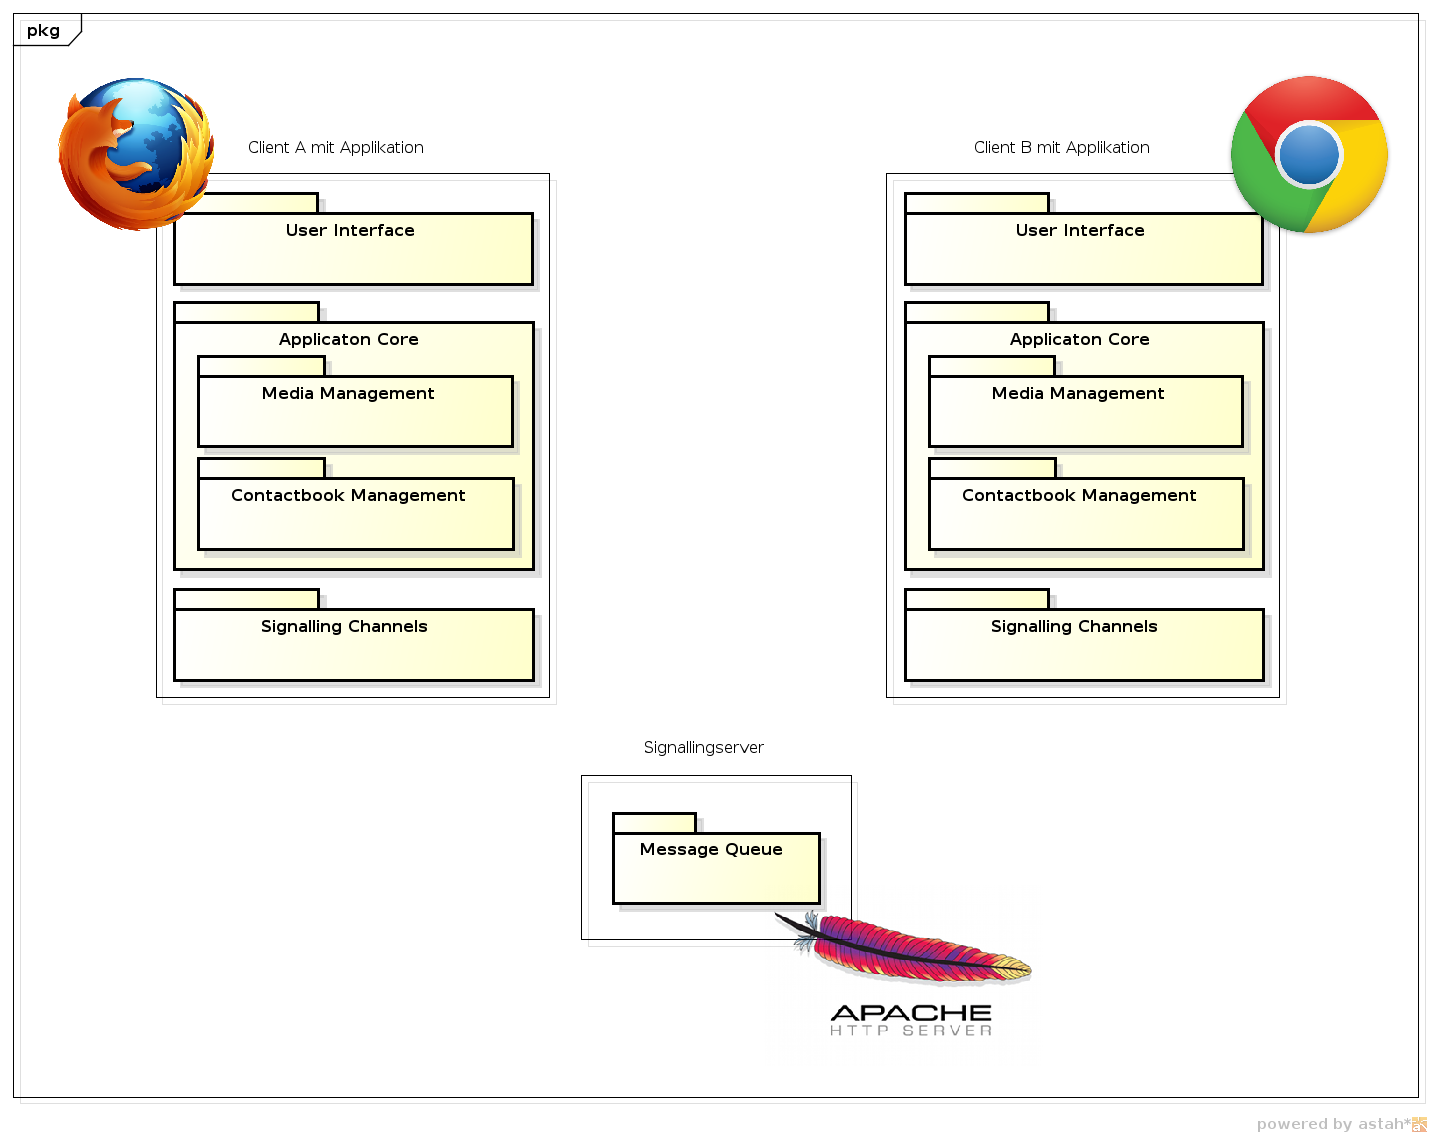
\includegraphics[width=1\textwidth]{../architekturanalayse/img/bigPicture.png}
		\caption{Big Picture JS VoIP App}
	\end{figure}
	Das Diagramm zeigt die erforderlichen Komponenten anhand zweier Clients. Jeder Client besitzt ein User Interface über welches der User die Kommunikation starten und beenden sowie Kontakbücher verwalten kann.
	
	$\rightarrow$ User Interface siehe Anhang \ref{uiDrafts}
	
	Jeder Client besitzt Signaling Channels, die mit einem Signaling Server interagieren. Hier wurde als Beispiel eine Message Queue auf einem Apache Server verwendet. Die Kommunikation läuft entsprechend über XHR.
	
	Für das Media Handling und die P2P-Kommunikation besitzt jeder Client ein Mediamanagement, das den P2P-Channel verwaltet und auf die lokale Mediaschnittstelle zugreift.
	

\section{Architektur-Detailmodell}
	Der logische Aufbau der Software besteht aus vier Schichten:
	\begin{figure}[H]
		\centering
		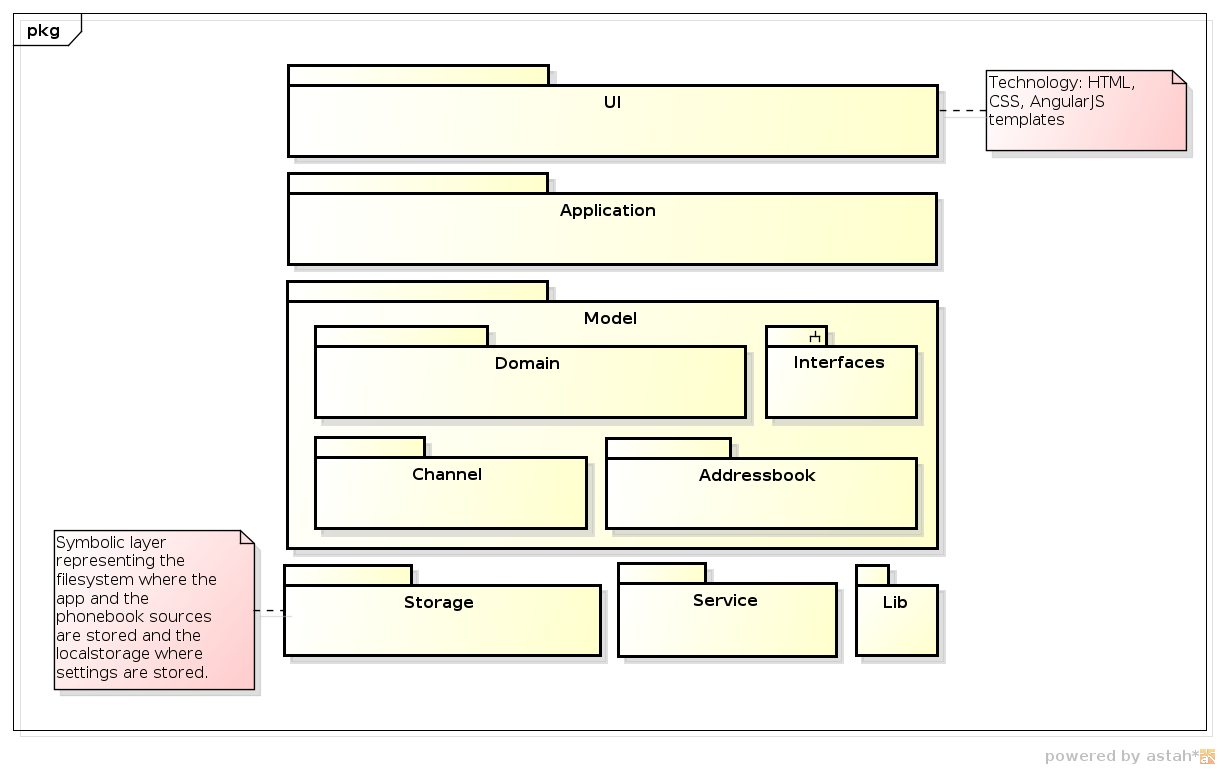
\includegraphics[width=1\textwidth]{../architekturanalayse/img/architecture.png}
		\caption{Architekturdiagramm JS VoIP App}
	\end{figure}
	Im untersten Layer sind Services und Libraries enthalten, auf die die oberen Layer zugreifen.
	Der Application Layer beinhaltet View Models für das User Interface und interagiert mit dem Model.
	

\begin{landscape}
\section{Domain}
	Im folgenden Diagramm sind die wichtigsten konzeptionellen Klassen und ihre Beziehungen untereinander aufgeführt.
	\begin{figure}[H]
		\centering
		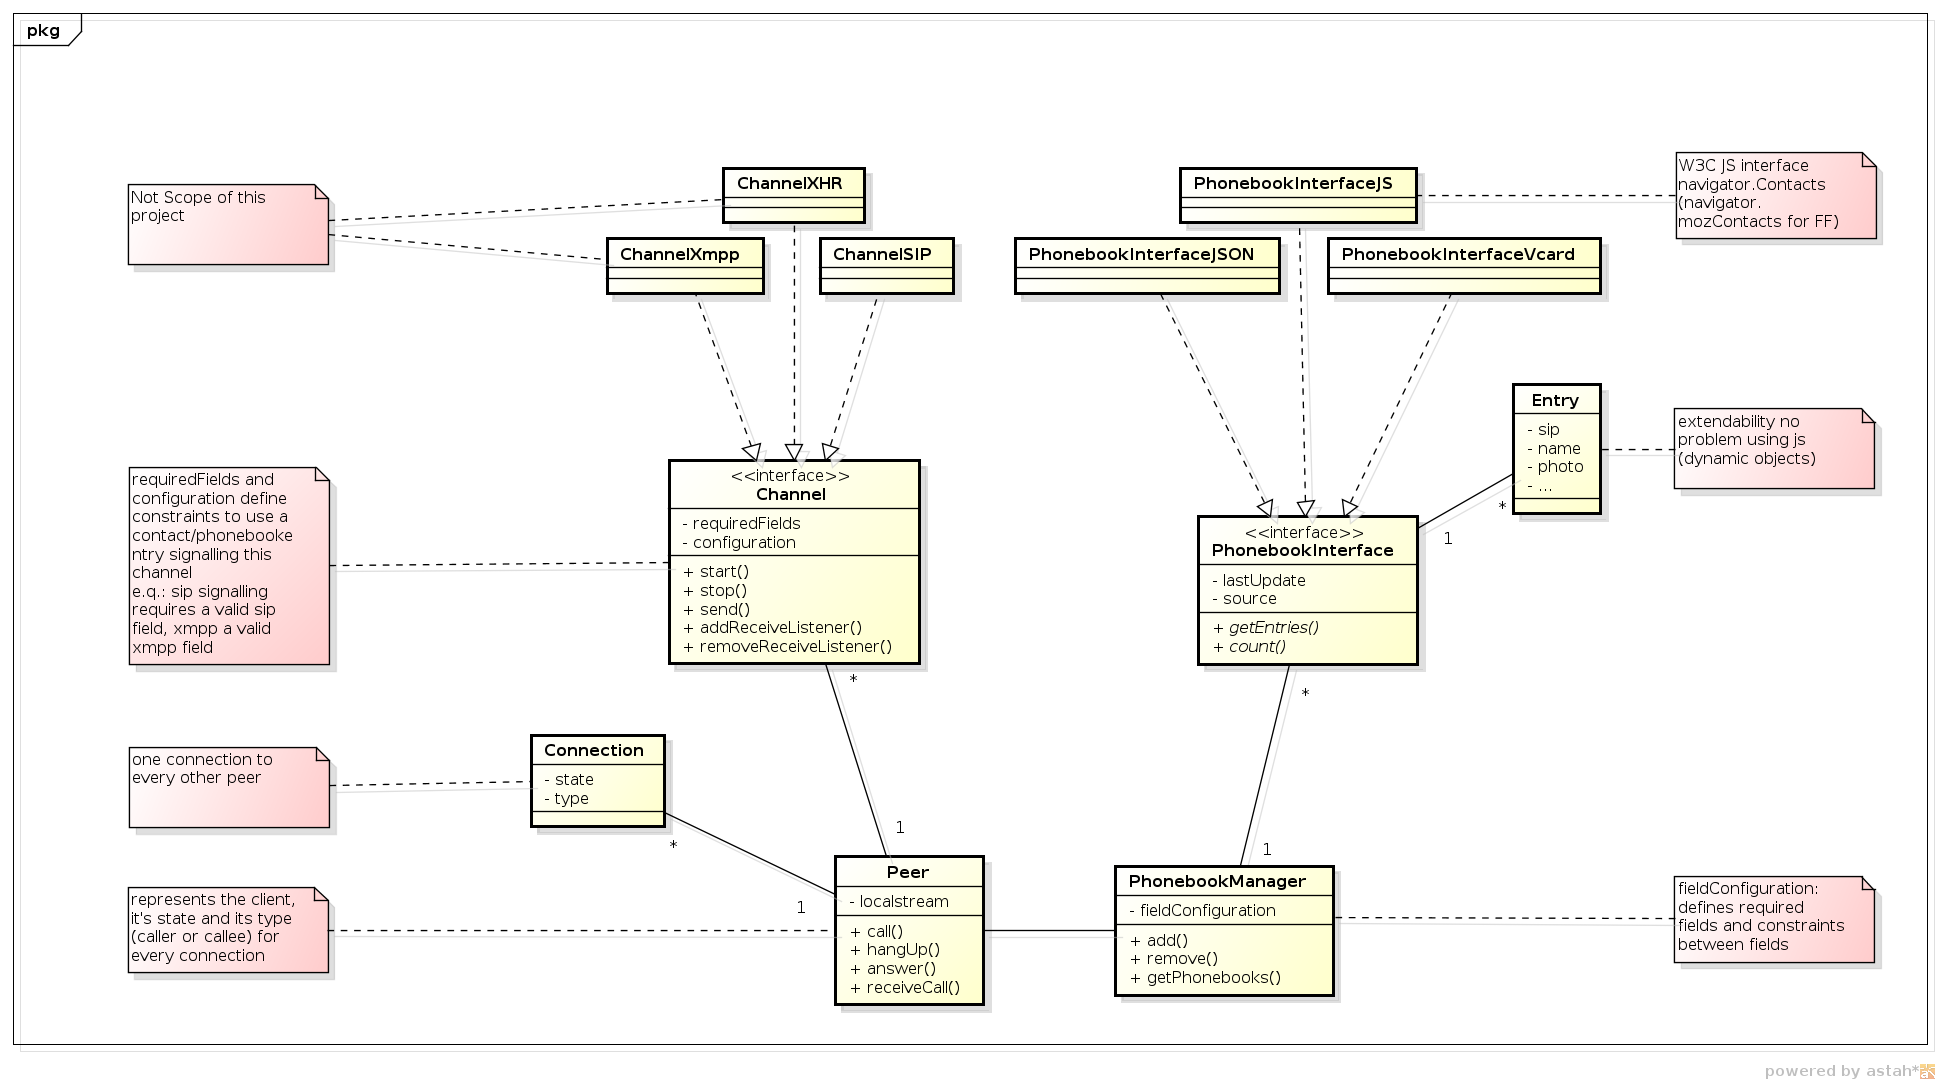
\includegraphics[width=1.2\textwidth]{../architekturanalayse/img/domain.png}
		%\caption{Strukturdiagramm JS VoIP App}
	\end{figure}
	Herzstück der Applikation sind die Channels und die Connection sowie das Contactbookmanagement.
	
	Die Channels laufen im Hintergrund und verbinden den User mit einem oder mehreren Signaling-Servern. Sie werden beim Login des Benutzers gestartet und müssen entsprechend ein Channel-Interface implementieren.
	
	Die Connection übernimmt das komplette Handling der P2P-Verbindung inklusive Verbindungsauf- und -abbau. Sie greift über den Host auf die lokale Kamera zu und sendet und empfängt über einen Channel "`Offers"' und "`Answers/Replies"'.
	
	Die Kontaktverwaltung übernimmt der ContactbookManager. Er importiert Kontaktbücher anhand der Konfiguration von den Quelle "`Datei"', "`Ordner"' oder "`Online"'. Für die formatspezifischen Importprozesse sind die jeweiligen Kontaktbücher zuständig. Dazu müssen alle Kontaktbücher das Addressbook-Interface umsetzen.
\end{landscape}
\clearpage

\section{Architektur-Designmotivations}
	\subsection{Client/Server vs. reine Client-Applikation}
		\subsubsection{Vorteile Client/Server-Umsetzung}
		\begin{itemize}
			\item Schlanker Client
			\item Es wird nur eine Schnittstelle benötigt zwischen Client und Server, der gesamte Verkehr kann über HTTP abgewickelt werden.
			\item Nur der Server muss die Schnittstellen zu anderen Diensten
			unterstützen. Keine zusätzlichen Schnittstellen-Anforderungen an den Client.
			\item Es ist einfacher durch Firewalls durchzukommen, da die Kommunikation genau kontrolliert werden kann.
		\end{itemize}
		\subsubsection{Nachteile}
		\begin{itemize}
			\item Redundanzen, da Funktionalität zwischen Client und Server durch
			ein eigenes Protokoll abgebildet und damit auf beiden Seiten Teile derselben
			Funktionalität umgesetzt werden müssen.
			\item Ein Anwender ist an den Server oder die Serverimplementation gebunden.
			Die Applikation läuft nicht ohne den Server.
			\item Der Server ist ein "`Single Point of Failure"'.
			\item Sollen weitere Schnittstellen umgesetzt werden, so muss der Server
			erweitert werden, was aufwendiger ist, als den Client zu erweitern.
		\end{itemize}


		\subsubsection{Vorteile reine Client-Lösung}
		\begin{itemize}
			\item Es wird kein Server benötigt.
			\item Anwender können einen beliebigen Kommunikationsserver
			(beispielsweise SIP\footnote{Session Initiation Protocol} oder
			XMPP\footnote{Extensible Messaging and Presence Protocol}) für das
			Signaling verwenden und sogar selbst eine eigene Channelimplementation
			hinzufügen.
			\item Um die Applikation für weitere Schnittstellen zu erweitern sind keine
			Kenntnisse der Servertechnologie notwendig.
			\item Die Applikation ist insgesamt weniger aufwändig aufgebaut, da sie
			weniger Redundanzen beinhaltet.
			\item Es ist keine eigene SIP-/XMPP-Server-Implementation erforderlich
			(bereits vorhandene Serverinfrastrukturen werden genutzt).
		\end{itemize}
		\subsubsection{Nachteile}
		\begin{itemize}
			\item Die möglichen Schnittstellen sind auf die Browserfunktionalität
			begrenzt (HTTP, WebSockets, RTSP\footnote{Realtime Strem Protocol}). Dadurch
			muss ein SIP- oder XMPP-Provider WebSockets unterstützen, damit er für das
			Signaling genutzt werden kann.
			\item Der Client wird umfangreicher.
			\item Probleme mit Firewalls und Routern möglich, die WebSocket-Pakete nicht
			weiterleiten. WebSockets können grundsätzlich über einen beliebigen Port laufen, meist wird jedoch Port 80 verwendet.
			\item Performanceprobleme möglich, da sämtliche Logik, inklusive dem Parsen
			der verschiedenen Protokolle, vom Client abgearbeitet werden muss.
		\end{itemize}

		\subsubsection{Fazit}
			Aufgrund geringerer Abhängigkeiten und der Wahrscheinlichkeit, das die
			SIP-Server-Provider irgendwann WebSockets unterstützen, wird die Lösung
			"`reine Client Applikation"' gewählt.
			Für die Kommunikation mit Signalingservern, wie SIP oder XMPP, werden
			WebSockets eingesetzt, für das Signaling über XHR\footnote{XmlHTTPRequest}
			wird mit der Option "`Allow Cross Origin"' gearbeitet.

	\subsection{STUN-Service}
		STUN\footnote{Session Traversal Utilities for NAT}-Services sind zwingend
		notwendig, um die nach aussen sichtbare IP-Adresse des Clients herauszufinden.
		Neben der Möglichkeit, selbst einen STUN-Service aufzusetzen, gibt es frei
		verfügbare STUN-Services, beispielsweise von Mozilla oder Google.

		Für ein abgeschottetes Netz ist ein eigener STUN-Server zwingend notwendig.
		Für unseren Fall reichen die frei verfügbaren. Durch anpassen der
		Konfiguration ist es möglich, den Server festzulegen.

		Im Netz gibt es fertig konfigurierte virtuelle Maschinen mit einsatzbereitem
		STUN-Service\footnote{Mozilla, stun-vm (Stand: 15.01.13). \hyperlink{https://github.com/mozilla/stun-vm}{https://github.com/mozilla/stun-vm} [Abgerufen am 28.10.13]}.

	\subsection{SIP-Proxy vs. SIP-Server mit WebSockets}
		Unterstützt ein SIP-Server keine WebSockets, so kann ein SIP/WebSocket-Proxy
		dazwischen geschaltet werden. Die Konfiguration eines SIP-Proxies ist ähnlich
		aufwändig wie die Installation eines Kamailio\footnote{Kamailio SIP Server
		Project, Features (Stand: 18.03.2013).
		\hyperlink{http://www.kamailio.org/w/features/}{http://www.kamailio.org/w/features/}, [Abruf am 28.10.13]}-SIP-Servers, der in der neusten Version WebSockets unterstützt.

	\subsection{Sicherheit}
		WebRTC-Streams können nur verschlüsselt übertragen werden. Es gibt keine
		Möglichkeit, die Verschlüsselung abzuschalten. Dies führt zwar zu einem
		erhöhten Rechenbedarf auf dem Client, garantiert jedoch eine verschlüsselte
		Verbindung unabhängig von den Vorlieben des Entwicklers.
		Die Verschlüsselung erfolg über DTLS-SRTP\footnote{IETF, RFC5764 (Stand: 2010). \hyperlink{http://tools.ietf.org/html/rfc5764}{tools.ietf.org/html/rfc5764}, [Abruf am 28.10.13]} keyings\footnote{Adam Roach, WebRTC: Security and Confidentiality (Stand: 07.06.13). \hyperlink{http://sporadicdispatches.blogspot.ch/2013/06/webrtc-security-and-confidentiality.html}{http://sporadicdispatches.blogspot.ch/2013/06/webrtc-security-and-confidentiality.html}, [Abruf am 28.10.13]}. 
		
		Die Verschlüsselung des Signaling-Channels ist abhängig von der eingesetzten
		Technologie. Werden z.B. Secure Websockets oder XHR über HTTPS eingesetzt so ist die Kommunikation verschlüsselt und nicht abgreifbar.
		
		Trotzdem kann ein Provider oder ein Geheimdienst Metadaten darüber sammeln, wer mit wem telefoniert.
		  
	\subsection{Hosting}
		Die JS-VoIP-App kann sowohl lokal, als auch von einem
		Webserver ausgeliefert ausgeführt werden. Es gibt keine speziellen Voraussetzungen. Ein Webserver ist daher nicht zwingend notwendig.
		

\clearpage
\section{Kommunikation}
	Die Kommunikation zwischen zwei Clients, einem STUN-Service und einem
	Signaling-Service wird im folgenden Diagramm dargestellt.
	\begin{figure}[H]
		\centering
		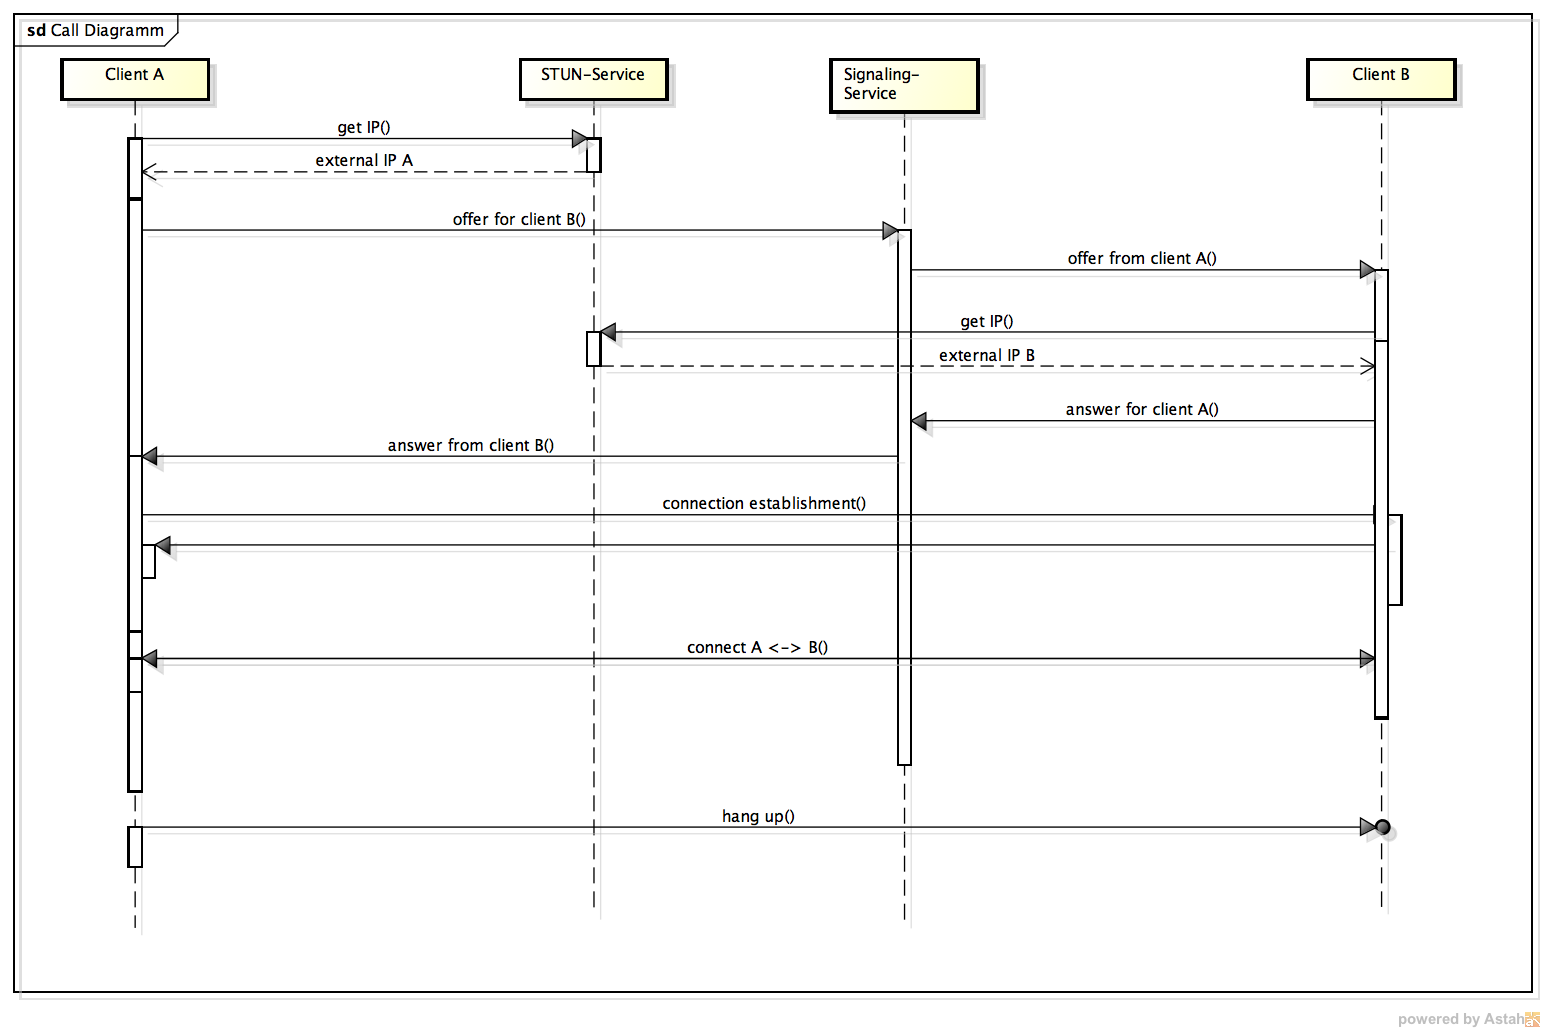
\includegraphics[width=\textwidth]{../architekturanalayse/img/callDiagramm.png}
		\label{img:deployment}
		\caption{Clientkommunikation}
	\end{figure}
	Die Clients beziehen vom STUN-Service ihre extern sichtbare IP und
	kommunizieren nach einem erfolgreichen Verbindungsaufbau direkt P2P ohne noch
	über den Signaling-Service zu gehen.
	
	Der Verbindungsabbau kann wahlweise über den Signaling-Server oder direkt P2P
	gesendet werden.
	
	
	\begin{landscape}		
		\begin{figure}[H]
			\centering
			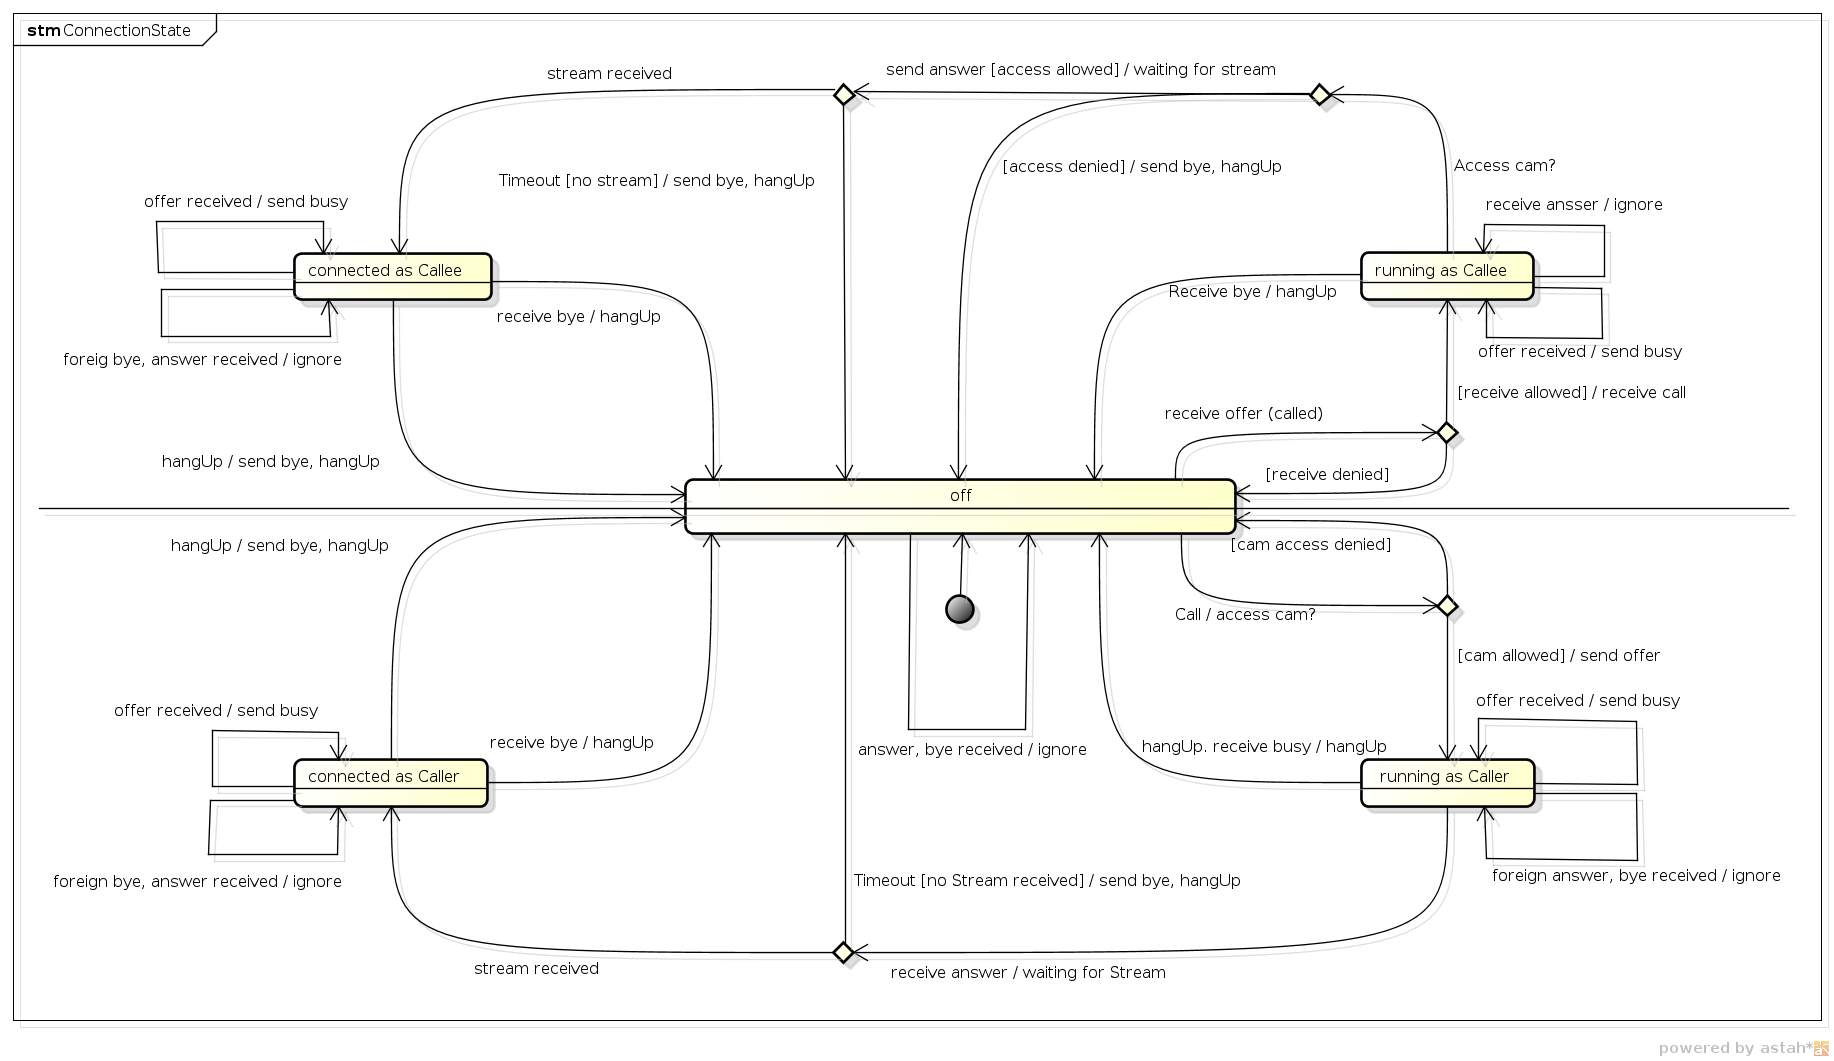
\includegraphics[height=0.7\textwidth]{../architekturanalayse/img/connectionState.png}
			\label{img:deployment}
			\caption{Applikationszustände}
		\end{figure}
		Beim Verbindungsaufbau nimmt jeder Client entwerde die Rolle "`Caller"' oder
		"`Callee"' ein. Erlaubt der Benutzer Zugriff auf die Kamera, so wird die
		Verbindung aufgebaut und bleibt bestehen, bis einer der Clients die Verbindung mit einem "`bye"' beendet.
		
		Ungültige Messages werden ignoriert. "`bye"' führt in jedem Zustand zu einem
		Abbruch der Verbindung bzw. des Aufbaus, vorausgesetzt das "`bye"'
		kommt vom anderen Kommunikationspartner.
	\end{landscape}
		
	
\clearpage
\section{Deployment}
	\begin{figure}[H]
		\centering
		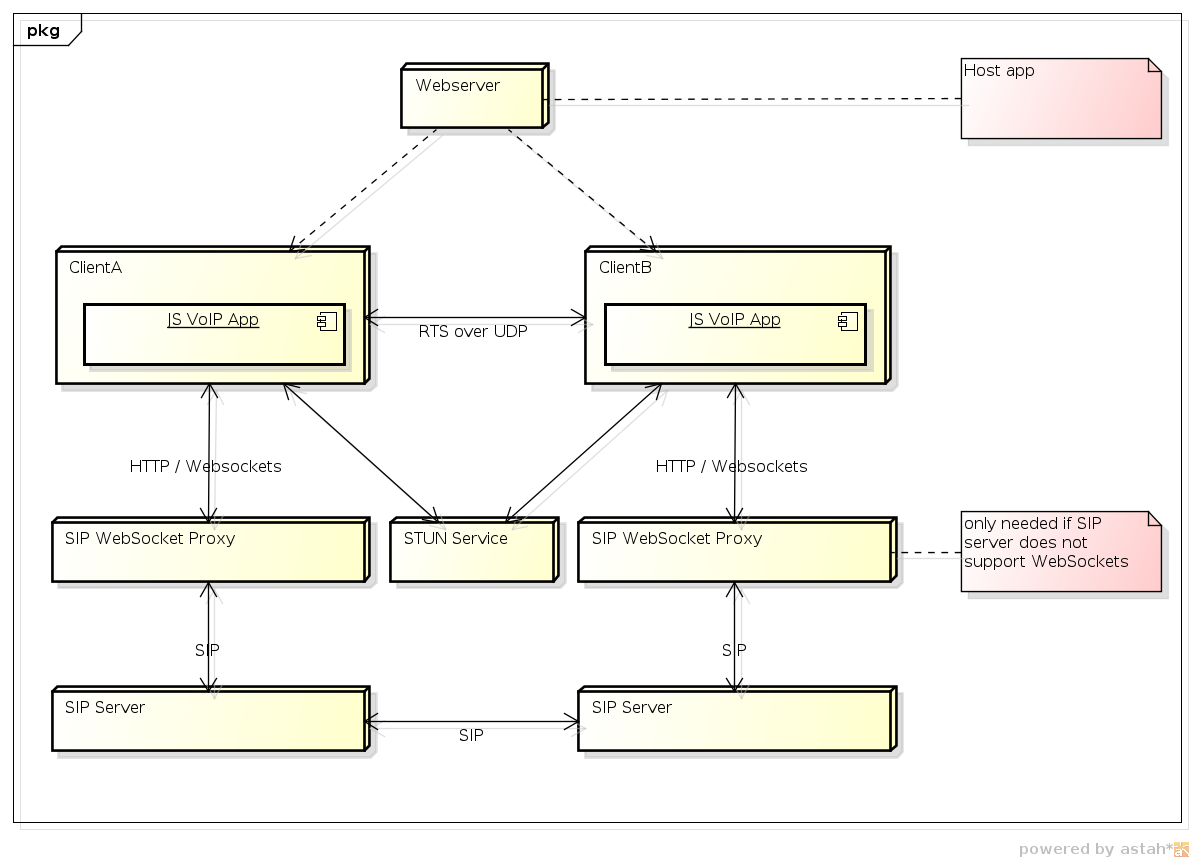
\includegraphics[width=\textwidth]{../architekturanalayse/img/deployment.png}
		\label{img:deployment}
		\caption{Deploymentdiagramm JS VoIP App}
	\end{figure}
	